\documentclass[a4paper,UTF8]{article}
\usepackage{ctex}
\usepackage[margin=1.25in]{geometry}
\usepackage{color}
\usepackage{graphicx}
\usepackage{amssymb}
\usepackage{amsmath}
\usepackage{amsthm}
\usepackage{listings}


%\usepackage[thmmarks, amsmath, thref]{ntheorem}
\theoremstyle{definition}
\newtheorem*{solution}{Solution}
\newtheorem*{prove}{Proof}
\usepackage{multirow}
\usepackage{url}
\usepackage[colorlinks,urlcolor=blue]{hyperref}
\usepackage{enumerate}
\renewcommand\refname{参考文献}

\usepackage{color}

\definecolor{dkgreen}{rgb}{0,0.6,0}
\definecolor{gray}{rgb}{0.5,0.5,0.5}
\definecolor{mauve}{rgb}{0.58,0,0.82}

\lstset{ %
  language=python,                % the language of the code
  basicstyle=\footnotesize,           % the size of the fonts that are used for the code
  numbers=left,                   % where to put the line-numbers
  numberstyle=\tiny\color{gray},  % the style that is used for the line-numbers
  stepnumber=2,                   % the step between two line-numbers. If it's 1, each line 
                                  % will be numbered
  numbersep=5pt,                  % how far the line-numbers are from the code
  backgroundcolor=\color{white},      % choose the background color. You must add \usepackage{color}
  showspaces=false,               % show spaces adding particular underscores
  showstringspaces=false,         % underline spaces within strings
  showtabs=false,                 % show tabs within strings adding particular underscores
  frame=single,                   % adds a frame around the code
  rulecolor=\color{black},        % if not set, the frame-color may be changed on line-breaks within not-black text (e.g. commens (green here))
  tabsize=2,                      % sets default tabsize to 2 spaces
  captionpos=b,                   % sets the caption-position to bottom
  breaklines=true,                % sets automatic line breaking
  breakatwhitespace=false,        % sets if automatic breaks should only happen at whitespace
  title=\lstname,                   % show the filename of files included with \lstinputlisting;
                                  % also try caption instead of title
  keywordstyle=\color{blue},          % keyword style
  commentstyle=\color{dkgreen},       % comment style
  stringstyle=\color{mauve},         % string literal style
  escapeinside={\%*}{*)},            % if you want to add LaTeX within your code
  morekeywords={*,...}               % if you want to add more keywords to the set
}

%--

%--
\begin{document}
\title{\textbf{《计算机图形学》3月报告}}
\author{181240004,曾许曌秋,\href{mailto:181240004@smail.nju.edu.cn}{181240004@smail.nju.edu.cn}}
\maketitle

\section{综述}
本月刚开始进行图形学大作业,主要完成了线段、多边形以及椭圆的算法实现以及相应的交互界面(顺便加上了我主页的icon)

\section{算法介绍}
\subsection{DDA}
DDA算法相比naive,只是对斜率$k>1$和$k<1$两种Case进行了分类讨论,当$k<1$时,沿x方向扫描,而$k>1$时则是沿着y方向扫描。从而避免了naive算法可能遇到的如图\ref{fig1}中k较大时像素点稀疏的情况
\begin{figure}[h]
    \centering
    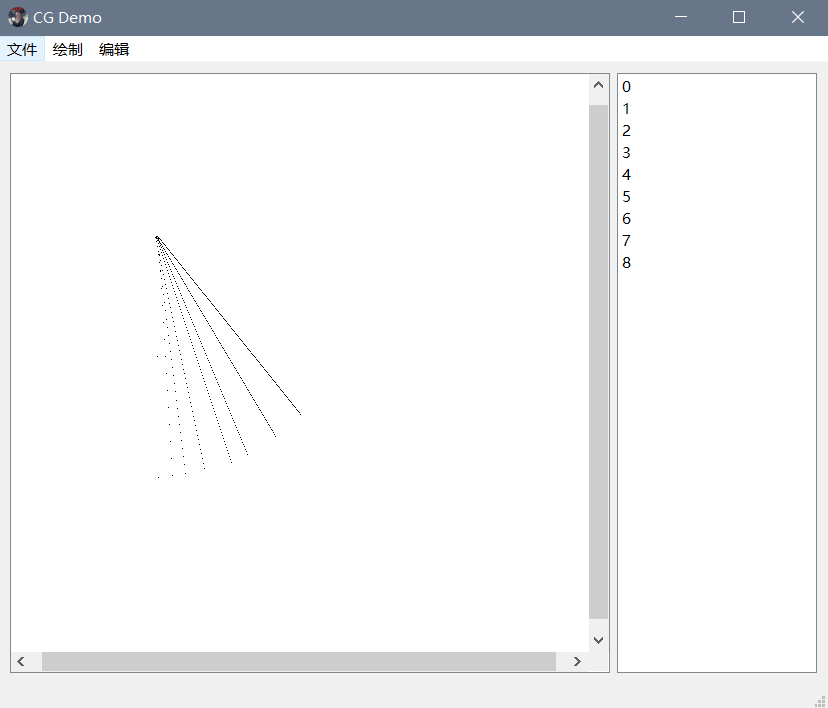
\includegraphics[width = .5\textwidth]{./source/pics/alg_naive.PNG}
    \caption{naive perform bad in the case that $k>1$}
    \label{fig1}
\end{figure}
\par
如图\ref{fig2}是DDA实现结果的演示,显然没有这个问题。
\begin{figure}
    \centering
    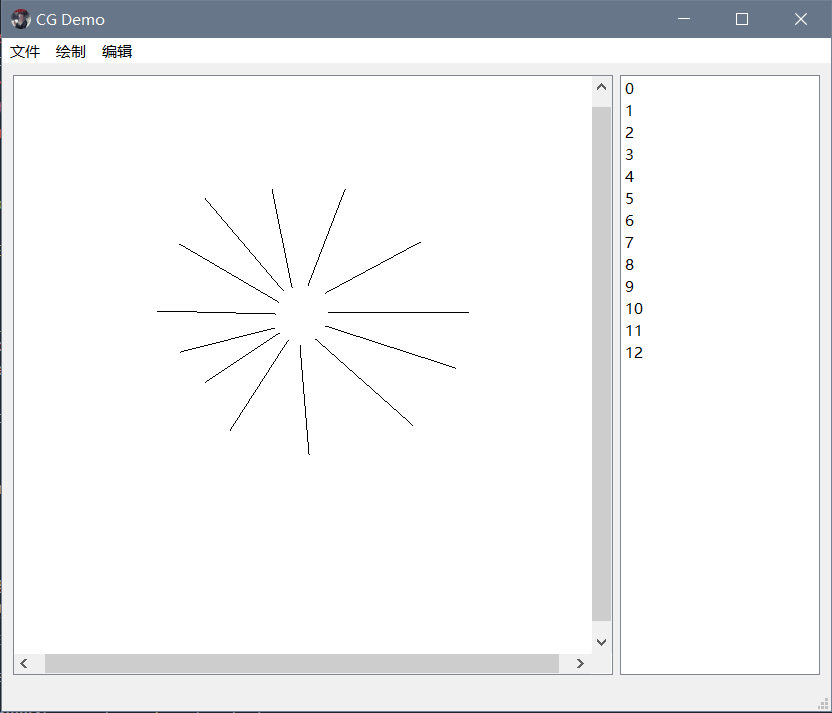
\includegraphics[width = .5\textwidth]{./source/pics/alg_dda.PNG}
    \caption{demonstration of DDA algorithm}
    \label{fig2}
\end{figure}

\subsection{Bresenham}
DDA算法中对每一个扫描方向坐标(x为例),另一个方向坐标(y)通过直接的暴力求出然后取‘int'的做法效率很低。
Bresenham算法则是通过动态维护(假定沿x方向扫描,即x方向斜率$\in (0, 1)$,当前位置(x, y))(x+1, y)处的整型判别式,从而保证基本只需要做整形的加减就可以完成扫描线。
演示如图\ref{fig3}
$$
\begin{aligned}
    determination = 2x\Delta y - (2y+1)\Delta x
\end{aligned}
$$
\begin{figure}[h]
    \centering
    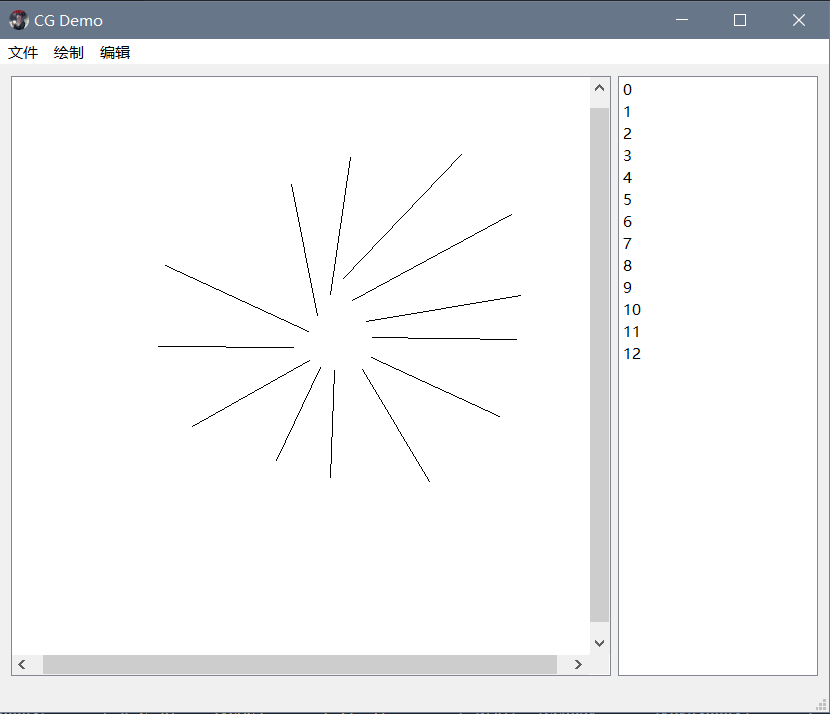
\includegraphics[width = .5\textwidth]{./source/pics/alg_bresenham.PNG}
    \caption{demonstration of Bresenham algorithm}
    \label{fig3}
\end{figure}

\subsection{Polygon}
多边形的实现显然(只要首位用线段相连即可,主要内容在交互界面,参考系统介绍部分)

\subsection{中点圆 - 椭圆}
对于圆而言,由对称性,只需要完成1/8然后关于圆心对称即可,而对于椭圆不妨只实现第一象限,其他象限对称即可。
\par
而对于第一象限而言,参考线段的实现方法,可以分为斜率绝对值大于1和小于1的两段分别沿x方向和y方向扫描,模范Bresenham算法,算出x方向扫描起点、整型椭圆判别式、斜率判别式及两个判别式的差分如下
$$
\begin{aligned}
    r_{start} &= ( \frac{x_{min} + x_{max} + 1}{2} , y_{max})\\
    p_{elli}(x, y) &= \Delta y^2 (2x - x_{sum})^2 - \Delta x^2 (2y-1-y_{sum})^2 \\
                & - \Delta x^2 \Delta y^2\\
    p_{slope}(x, y) &= \Delta x^2(2y-1-y_{sum}) - \Delta y^2(2x - x_{sum})\\
    p_{elli}(x+1, y-\frac{1}{2}) - p_{elli}(x, y-\frac{1}{2}) &= 4\Delta y^2(2x+1 -x_{sum})\\
    p_{elli}(x+1, y-\frac{1}{2}) - p_{elli}(x, y+\frac{1}{2}) &= 4\Delta y^2(2x+1 -x_{sum}) - 4\Delta x^2(2y -y_{sum})
\end{aligned}
$$
\par

\begin{lstlisting}
    # walk by a
    def ellipse_walk(amin, amax, bmin, bmax, loc):
        resulta = []
        asum = amin + amax; da = amax - amin; da_sq = da*da
        bsum = bmin + bmax; db = bmax - bmin; db_sq = db*db
        a = (int) ( (asum + 1) / 2 )
        b = bmax
        walk = True
        p_slope = da_sq*(2*b - bsum) - db_sq*(2*a - asum)
        p_elli = db_sq*( (2*a + 2 - asum)**2 ) + da_sq*(1 - 2*db)  # 2*a - asum = 1 or 0 = ()*()  | a+1, b-1/2
        while walk:
            resulta.append( loc(a, b)   )
            resulta.append( loc(a, bsum-b)  )
            resulta.append( loc(asum-a, b)  )
            resulta.append( loc(asum-a, bsum-b) )
            if p_elli < 0:
                a = a + 1
                b = b
                p_elli = p_elli + 4*db_sq*(2*a + 1 - asum)
                p_slope = p_slope - 2*db_sq
            else:
                a = a + 1
                b = b - 1
                p_elli = p_elli + 4*db_sq*(2*a + 1 - asum) - 4*da_sq*(2*b - bsum)
                p_slope = p_slope  - 2*da_sq - 2*db_sq
            assert( p_elli == db_sq*(2*a + 2 - asum)**2 + da_sq*(2*b - 1 - bsum)**2 - da_sq*db_sq )
            walk = (p_slope > 0)
        return resulta
\end{lstlisting}
其中$\Delta x = x_{max} - x_{min}, x_sum = x_{max} + x_{min}$,效果如\ref{fig4}所示:
\begin{figure}[h]
    \centering
    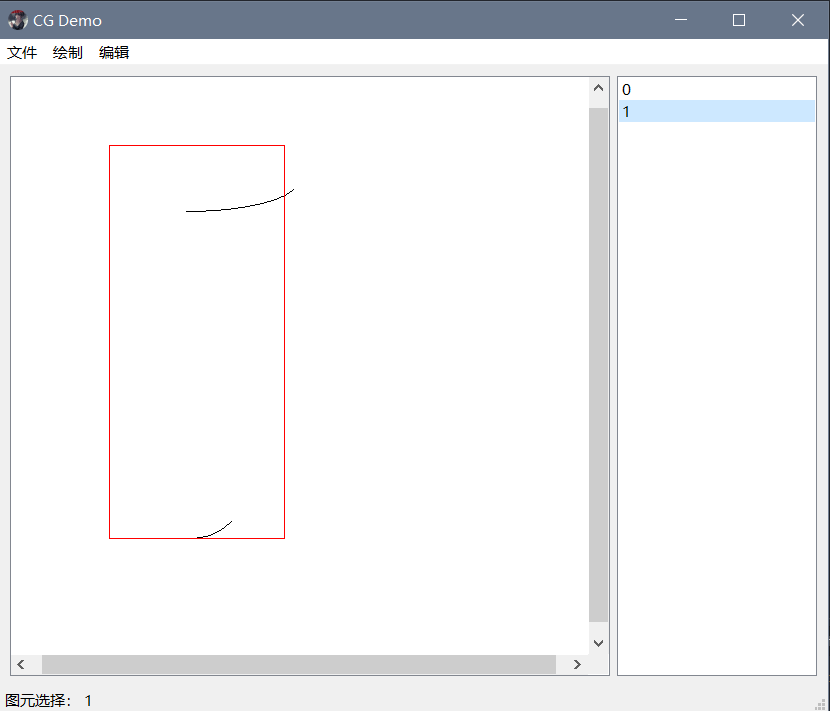
\includegraphics[width = .5\textwidth]{source/pics/circle_demon1.PNG}
    \caption{circle demon 1}
    \label{fig4}
\end{figure}

关于原点对称得到图\ref{fig5}:
\begin{figure}[h]
    \centering
    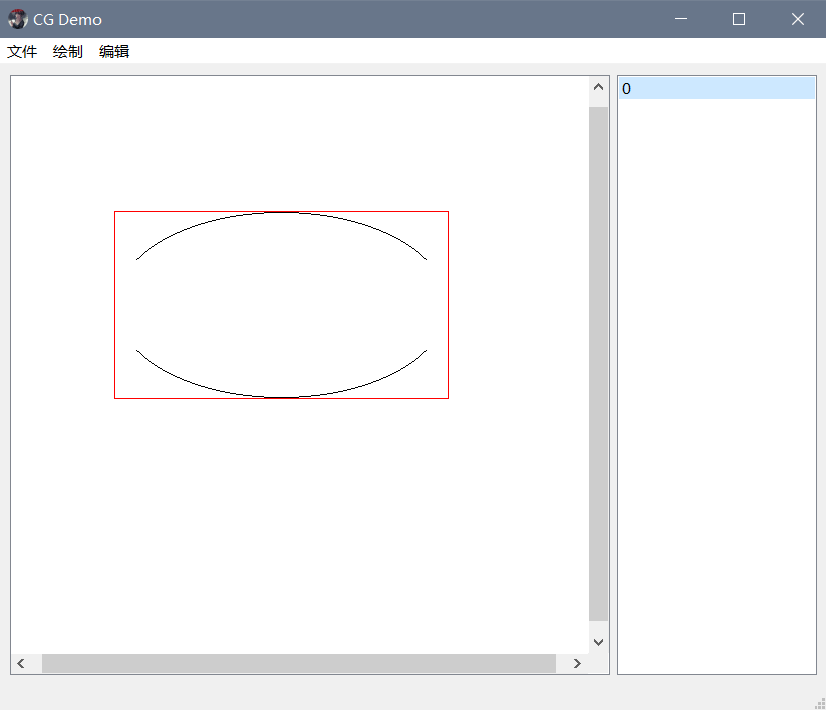
\includegraphics[width = .5\textwidth]{source/pics/circle_demon2.PNG}
    \caption{circle demon 2}
    \label{fig5}
\end{figure}

再沿y方向重复该操作即得椭圆\ref{fig6}
\begin{figure}
    \centering
    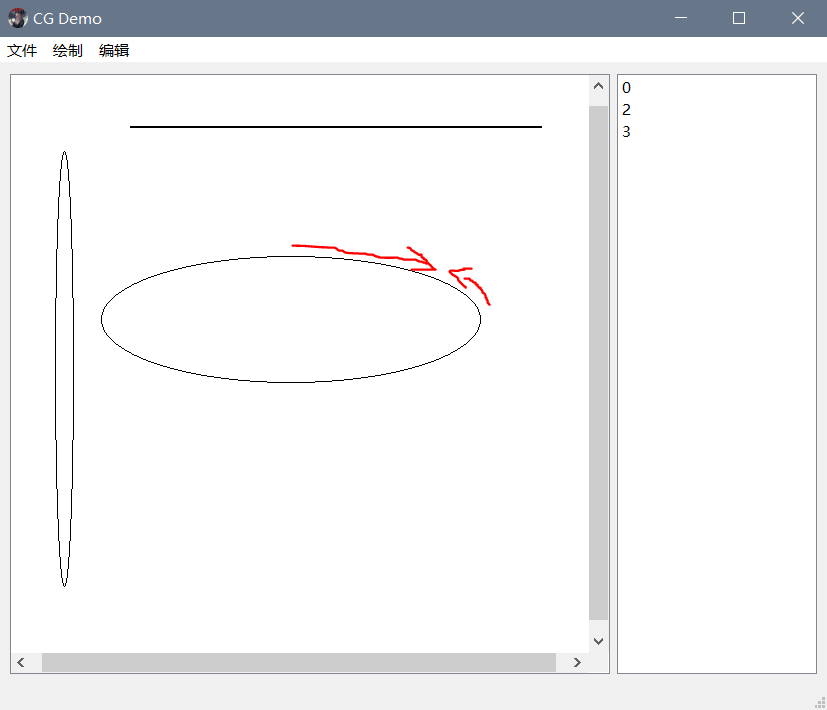
\includegraphics[width = .5\textwidth]{source/pics/circle_demon3.PNG}
    \caption{circle demon 3}
    \label{fig6}
\end{figure}

\subsection{优雅的代码}
注意到DDA、Bresenham以及中点圆都存在大量的对称性(x、y的交换对称性,x、y轴的对成性)暴力分类讨论会造成冗长且不易维护的代码。
通过使用一个简单的“switch”函数和三元表达式即可实现核心算法部分代码的复用性:
\begin{lstlisting}
    def noswitch(x, y):
        return (x, y)

    def switch(x, y):
        return (y, x)

    if abs(x1 - x0) > abs(y1 - y0): # walk by x
        loc = noswitch
        (a0, b0, a1, b1) = (x0, y0, x1, y1) if x0 < x1 else (x1, y1, x0, y0)
    else:           # walk by y (containing the special case)
        loc = switch
        (a0, b0, a1, b1) = (y0, x0, y1, x1) if y0 < y1 else (y1, x1, y0, x0)
    # s.t a0 <= a1 && abs(a1 - a0) >= abs(b1 - b0)
    # algorithm here
\end{lstlisting}

\par
中点圆同理
\begin{lstlisting}
    x0, y0 = p_list[0]
    x1, y1 = p_list[1]
    (xmin, xmax) = (x0, x1) if x0 < x1 else (x1, x0)
    (ymin, ymax) = (y0, y1) if y0 < y1 else (y1, y0)
    return ellipse_walk(xmin, xmax, ymin, ymax, noswitch) \
         + ellipse_walk(ymin, ymax, xmin, xmax, switch)
\end{lstlisting}

		
\section{系统介绍}
交互界面基本上只有多边形(polygon)需要单独考虑,目前的交互方式是鼠标按下开始绘制,鼠标移动会拖拽当前vertex,从开该vertex会确认,同时新建一个vertex,右键从开退出绘制。因为多边形的特殊交互性质,为画布添加了额外状态变量is\_drawing。

\subsection{好看的界面}
目前还只有一个icon

\section{总结}
因为才开始做,仅仅只实现了几个基本算法及其交互界面

\bibliographystyle{plain}%
%"xxx" should be your citing file's name.
\bibliography{}

\end{document}